\section{\label{sec:uncertainties}Systematic Uncertainties}
Multiple sources of systematic errors were investigated. Estimation procedures for beam and PIA$\nu$O detector systematics are unchanged from \cite{duet} and are briefly outlined in Sec. \ref{sec:beam_syst} and \ref{sec:piano_syst}. CEMBALOS detector systematics are summarized in Sec. \ref{sec:cembalos_syst}. Uncertainties related to the physics modeling are discussed in Sec. \ref{sec:physics_syst}. Table \ref{table:systematics} shows a summary of all the systematic uncertainties estimated for this analysis.

\begin{table*}[htbp]
\begin{center}
\begin{tabular*}{\textwidth}{l|@{\extracolsep{\fill}}ccccc|ccccc}
\hline\hline
& \multicolumn{5}{c}{CX} & \multicolumn{5}{c}{ABS} \\
\hline
{\bfseries$\pi^+$ Momentum [MeV/c]}& 201.6 & 216.6 & 237.2 & 265.5 & 295.1 & 201.6 & 216.6 & 237.2 & 265.5 & 295.1 \\
\hline
  {\bfseries Beam Systematics} & & & & &  & & & & &\\
  ~~Beam profile& 3.5& 4.9& 6.2& 4.2& 2.0& 2.2& 2.7& 3.8& 2.9& 2.5 \\
%  ~~Beam profile& 4.3& 9.0& 6.4& 3.7& 3.7& 2.6& 4.3& 4.3& 2.5& 1.9 \\
  ~~Beam momentum& 4.1& 1.6& 3.5& 4.1& 2.8& 1.5& 2.3& 1.9& 2.5& 3.0 \\
%  ~~Beam momentum& 4.5& 4.0& 3.7& 4.1& 2.0& 1.8& 2.4& 2.2& 2.1& 2.5 \\
  ~~Muon Contamination& 0.5& 0.8& 0.9& 0.3& 0.2& 0.5& 0.8& 0.9& 0.3& 0.2 \\
  \hline
  {\bfseries PIA$\nu$O Systematics} & & & & &  & & & & &\\
  ~~Fiducial volume& 3.6& 2.3& 4.3& 3.9& 4.5& 1.1& 5.4& 4.1& 3.8& 3.4 \\
  ~~Charge distribution& 3.3& 4.1& 3.3& 2.4& 3.0& 4.3& 3.2& 4.1& 4.1& 4.4 \\
%  ~~Charge distribution& 4.8& 6.0& 3.3& 3.0& 3.6& 4.8& 6.0& 3.3& 3.0& 3.6 \\
%  ~~Charge distribution& 5.2& 5.9& 11.0& 3.1& 5.0& 5.2& 5.9& 11.0& 3.1& 5.0 \\
  ~~Crosstalk probability& 3.9& 4.9& 4.4& 2.5& 2.2& 1.9& 2.0& 2.7& 1.7& 1.3 \\
%  ~~Crosstalk probability& 2.1& 1.9& 2.4& 1.2& 1.8& 1.6& 1.5& 1.9& 1.3& 1.1 \\
  ~~Layer alignment& 1.3& 3.6& 2.9& 0.9& 1.1& 1.0& 2.3& 2.8& 1.7& 2.4 \\
%  ~~Layer alignment& 1.3& 5.6& 3.0& 1.4& 0.9& 1.5& 2.5& 3.1& 2.3& 1.7 \\
  ~~Hit inefficiency& 1.0& 2.1& 2.1& 2.5& 2.6& 1.1& 1.3& 1.5& 2.0& 1.0 \\
  ~~Target material& 2.0& 2.0& 2.9& 2.9& 2.9& 1.2& 1.2& 1.2& 1.2& 1.3 \\
  \hline
  {\bfseries CEMBALOS Systematics} & & & & &  & & & & &\\
%  ~~Harpsichord Charge& 2.7& 2.9& 3.6& 4.1& 4.8& 1.5& 1.1& 1.9& 2.1& 1.8 \\
%  ~~Harpsichord Hit Inefficiency& 0.9& 0.8& 0.9& 0.7& 0.5& 0.9& 0.8& 0.9& 0.7& 0.5 \\
  ~~Charge calibration& 1.7& 1.6& 3.7& 3.1& 6.7& 1.3& 1.1& 2.0& 1.7& 2.5 \\
  ~~Hit inefficiency& 1.6& 2.1& 1.1& 1.3& 2.0& 1.2& 1.1& 1.1& 1.0& 0.9 \\
  ~~Position and alignment & 7.7& 7.9& 8.3& 5.7& 4.6& 0.7& 1.0& 0.7& 0.7& 1.0 \\
%  ~~Partial Sum & 8.1& 8.3& 9.2& 6.6& 8.4& 1.9& 1.9& 2.4& 2.1& 2.8 \\
  %~~Partial Sum& 8.2& 8.4& 9.1& 7.0& 4.6& 1.9& 1.6& 2.2& 2.3& 1.0 \\
  \hline
  {\bfseries Physics Systematics} & & & & &  & & & & &\\
%  ~~\st{Geant4$\sim$FLUKA thin target}& 22.0& 17.2& 14.2& 10.8& 5.7& 9.1& 4.2& 6.2& 5.1& 2.1 \\
  ~~$\pi^{0}$ kinematics& 6.1& 6.9& 7.9& 9.4& 10.6& 2.1& 1.6& 3.2& 4.3& 4.1 \\
  ~~Nuclear de-excitation $\gamma$ background& 0.9& 0.8& 0.7& 0.6& 0.6& 0.4& 0.2& 0.7 & 0.3& 0.2 \\
  ~~Multiple interactions& 1.1 & 1.9 & 1.7 & 1.5 & 1.8 & 0.5& 0.5& 0.8& 0.7& 0.7 \\
  ~~Pion decay background& 1.9 & 2.8& 1.2& 0.6& 0.9& 0.8& 0.7& 0.5& 0.3& 0.3 \\
  %~~Multiple interactions& 1.1& 1.9& 1.7& 1.5& 1.8& 1.1& 1.9& 1.7& 1.5& 1.8 \\
  %~~$\pi{+}$ decay background& 1.9& 2.8& 1.2& 0.6& 0.9& 1.9& 2.8& 1.2& 0.6& 0.9 \\
  \hline
  {\bfseries Statistical error} & 11.0& 26.0& 9.4& 8.9& 8.8& 3.9& 6.2& 3.9& 4.2& 3.6 \\
  \hline\hline
  %{\bfseries Total error} & 27.6& 34.1& 22.7& 17.8& 15.6& 12.0& 11.7& 11.8& 10.2& 9.1 \\
  %{\bfseries Total error} & 17.9& 30.3& 19.4& 17.0& 18.0& 8.0& 11.0& 10.5& 9.8& 9.8 \\
  {\bfseries ~~Total error} & 17.9& 30.3& 19.4& 17.0& 18.0& 7.8& 10.5& 10.4& 9.7 & 9.6 \\
  \hline
\end{tabular*}
\caption{Summary of the statistical and systematic uncertainties in percentage.}
\label{table:systematics}
\end{center}
\end{table*}

\subsection{Beam systematics}\label{sec:beam_syst}
The pion beam profile and momentum were measured using PIA$\nu$O through-going pion data. The uncertainties were less than $\sim$1 mm and $\sim$1 MeV$/c$, respectively. The systematic error was evaluated by changing the momentum, the center position, and the beam spread in the MC within their uncertainty and re-calculating the cross sections.
\subsection{PIA$\nu$O detector systematics}\label{sec:piano_syst}
Various sources of systematic uncertainty were estimated for PIA$\nu$O following the procedures described in \cite{duet}. These account for uncertainties on the scintillator fiber composition, the size of the fiducial volume, the alignment of the fibers, and the simulation of the charge deposition, hit detection efficiency, and crosstalk. For this analysis the same procedures were used.
\subsection{CEMBALOS detector systematics}\label{sec:cembalos_syst}
\subsubsection{\bf Position and alignment}
The overall uncertainty in the position of CEMBALOS relative to PIA$\nu$O, and of the position of the scintillator and lead modules relative to the dark box as well as each other is estimated to be $\pm$5 mm. This corresponds to a change of $\sim$3.4\% in the subtended solid angle. The effect to the calculated cross section is estimated by shifting the position of CEMBALOS in the simulation $\pm$ 5mm in the $x,y$, and $z$ directions. The relatively large size of this systematic uncertainty (4.5$\sim$8.3\%) is due to the sensitivity of this measurement to the $\pi^0$ kinematics and will be discussed in further detail in Sec. \ref{sec:physics_syst}.
\subsubsection{\bf Charge simulation}
The calibration procedure presented in Sec. \ref{section:calibration} and Fig. \ref{fig:muoncharge} show that for single hits from minimum ionizing particles ($<50$ p.e.) the charge simulation agrees with data at the $\sim5$\% level. However, as can be seen from Fig. \ref{fig:nhitsvsCharge}, for most of the background events the charge deposited per hit is above this region. A control sample of protons stopping in the first two XY modules of CEMBALOS was used to estimate the accuracy of the charge simulation for higher energy depositions. It was obtained by using $dQ/dx$ information from PIA$\nu$O to select ``proton-like'' tracks and requiring all CEMBALOS hits to be in the first two XY modules. Fig. \ref{fig:proton_sample} shows the charge deposition distribution in the first layer of CEMBALOS for this sample in data and MC.
\begin{figure}[ht]
 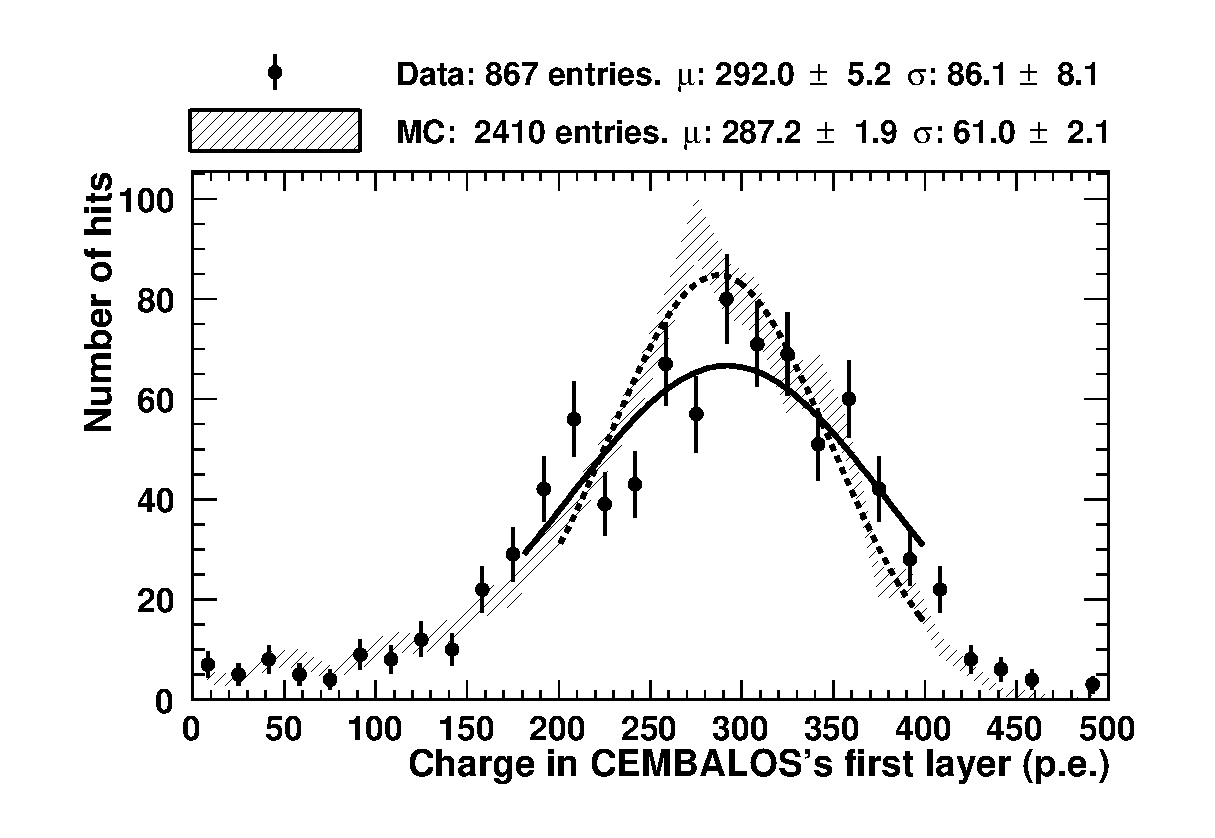
\includegraphics[width=86mm]{figures/proton_contained_1stlayer.eps}
 \caption{Charge distribution in the first layer of CEMBALOS for stopping protons in the 237.2 MeV$/c$ setting for data (circles) and MC (filled histogram). Only statistical uncertainties are plotted. The solid and dashed lines are Gaussian fits to data and MC respectively.}
 \label{fig:proton_sample}
\end{figure}

The discrepancy in the resolution for data and MC was estimated to be 20\% from the widths of Gaussian fits of the distributions in Fig. \ref{fig:proton_sample}.
{\color{red}A random Gaussian smearing with a 20\% width was applied to the charge deposited by each hit in every event for 1000 toy MC experiments to determine what fraction of the time signal events were mis-reconstructed as background and vice versa. The cross section was calculated for each toy experiment and the spread was taken as the uncertainty.}
%The systematic uncertainty was propagated to the cross section measurement by applying a Gaussian smearing with a 20\% width to the charge deposition per event in 1000 toy MC experiments.

\subsubsection{\bf Hit inefficiency}
The hit reconstruction inefficiency in CEMBALOS was measured by counting how often a hit was missing in a reconstructed track. The tracks were required to have at least two hits in both the first and last two layers. Fig. \ref{fig:hit_ineff} shows the hit inefficiency, defined as the ratio of missing hits over the total number of hits expected, for data and MC in the 237.2 MeV$/c$ setting as a function of the CEMBALOS reconstructed polar angle. The hit inefficiency integrated over all angles is 1.33\% and 1.16\% for data and MC respectively.
\begin{figure}[ht]
 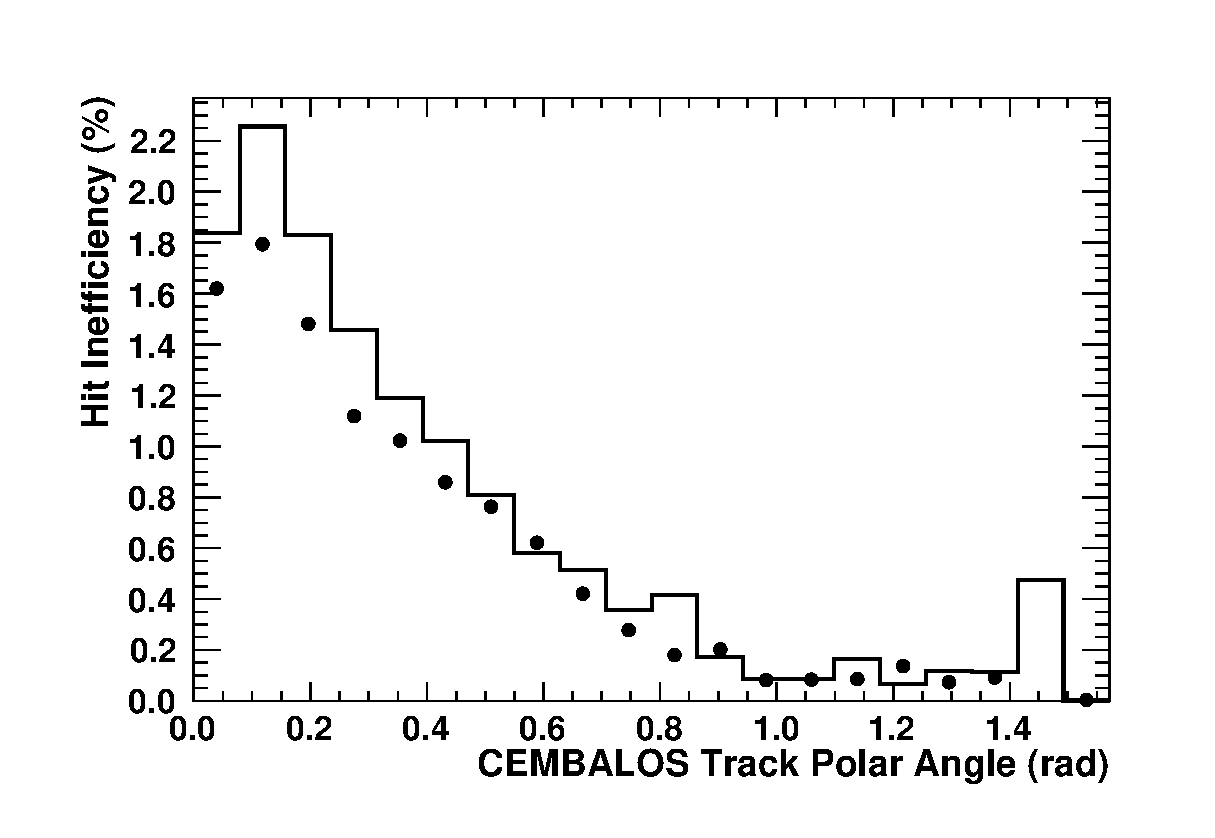
\includegraphics[width=86mm]{figures/cembalos_hit_ineff_237.eps}
 \caption{CEMBALOS hit inefficiency for data (circles) and MC (solid line) in the $p_\pi=$237.2 MeV$/c$ setting. The statistical error bars are too small to appear.}
 \label{fig:hit_ineff}
\end{figure}

The effect on the measured cross section is estimated by randomly deleting CEMBALOS hits in 1000 MC toy experiments with a probability given by the difference of the integrated hit inefficiencies for data and MC, affecting both the hit multiplicity and total charge deposited.

\subsection{Physics modeling systematics}\label{sec:physics_syst}
\subsubsection{\bf{ Uncertainty from $\pi^{0}$ kinematics }}
True CX events were reweighted following the discrepancy between \cite{Ashery2} and the \textsc{Fluka} model prediction as a function of the $\pi^{0}$ angle. The weights ranged from 0.7 to 1.3, while the average weight applied was 0.9. The effect on $\sigma_{\mathrm{CX}}$ ranged  from 6.1\% to 10.6\%, representing the largest systematic uncertainty for this analysis.

\subsubsection{\bf Other backgrounds}\label{sec:background}
The uncertainties from additional contributions to the number of predicted background events were estimated in three different categories, as described in the following text.

{ \it Nuclear de-excitation $\gamma$-rays:} inelastic interactions can leave the nucleus in an excited state. Low-energy ($<25$ MeV$/c$) $\gamma$-rays can be emitted as the nucleus returns to its ground state. If these photons interact in CEMBALOS they can fake a signal event. While these processes are believed to be well modeled by our simulation, we assign a conservative 100\% error on the number of background events from this process.\\

{ \it Multiple interactions: } it is possible for the initial $\pi^{+}$ to be scattered (both elastically or quasi-elastically) before it undergoes a CX interaction. The CX interaction can take place inside the PIA$\nu$O FV ($\sim$58\%), outside the FV but still in a scintillator fiber ($\sim$37\%), or somewhere in the aluminum support structure and/or dark boxes of PIA$\nu$O or CEMBALOS ($\sim$5\%). The uncertainty of the number of events of this type of background event is estimated from the uncertainty on elastic and CX interactions on carbon and aluminum from previous experiments.\\

{ \it $\pi^{+}$ decay products: } a $\pi^{+}$ that scatters in PIA$\nu$O and produces a fake ``proton-like'' track can then stop and decay around or inside CEMBALOS, possibly circumventing the veto rejection. The decay products can then deposit enough energy in CEMBALOS to produce a fake signal event. A conservative 100\% uncertainty is assigned to these events, which amount to $\sim$1\% of the selected events. %Fig. \ref{fig:ev_disp_decay} shows an example of these type of events

%\begin{figure}[ht]
%    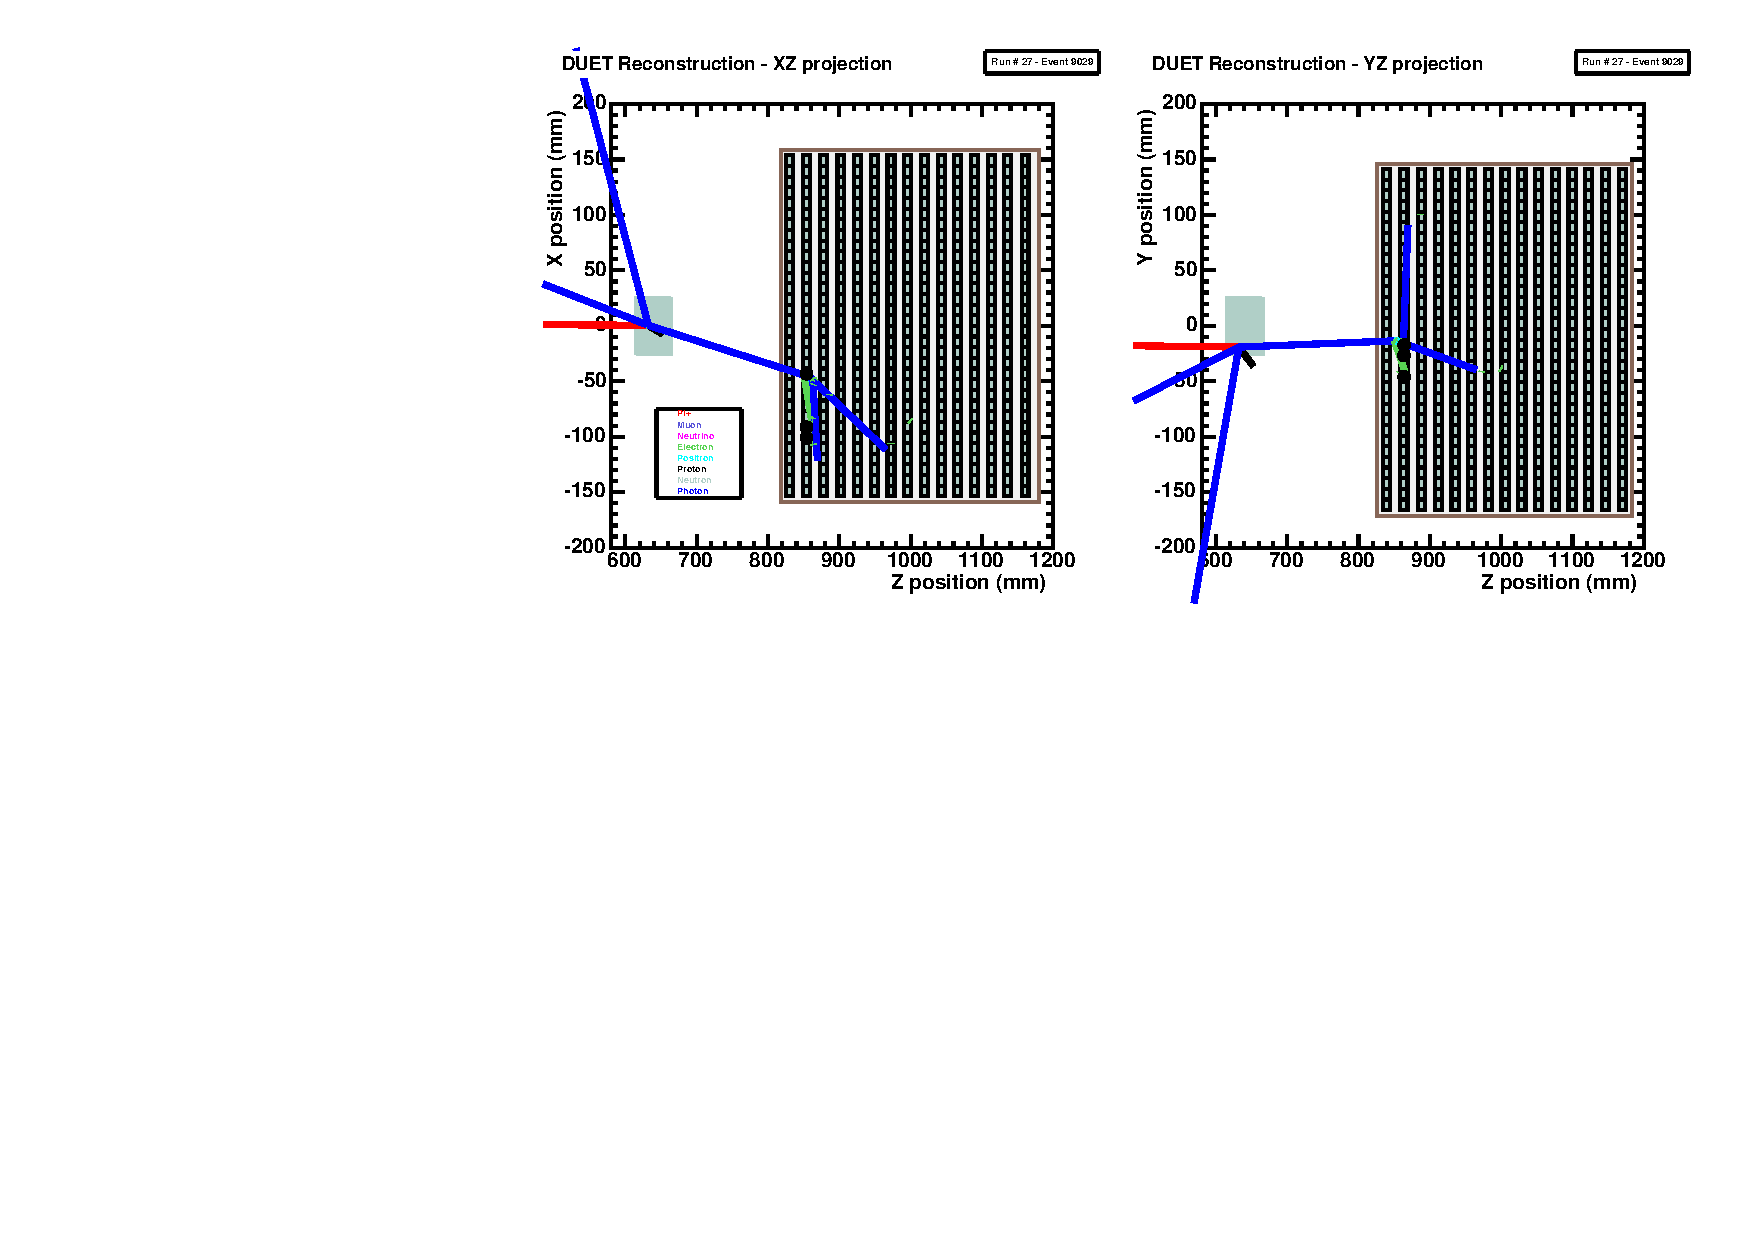
\includegraphics[width=90mm]{figures/ev_display_27_9029_intr4_ntag267.pdf}
%    \caption{Example of a CX event ($p_\pi=$237.2 MeV$/c$). A $\pi^+$ (red) undergoes CX in PIA$\nu$O resulting in a $\pi^0$ decay to two photons (blue). A forward-going photon is identified in CEMBALOS as it showers and hits are recorded in the scintillating material.}
%   \label{fig:ev_disp_decay}
%   \end{figure}

%\subsection{Summary of uncertainties}